% Points z_0, ..., z_6 on a slightly outward-spiralling arc (red) and their
% cubes z^3 (blue). As z sweeps 270 degrees around the origin, z^3 sweeps
% 810 degrees -- winding three times as fast, illustrating that z^n winds n
% times when z winds once.
% Source: book/tex/complex-ana/meromorphic.tex
%   (section: Digression: the Argument Principle viewed geometrically).
\documentclass[border=2mm]{standalone}
\usepackage{tikz}
\usetikzlibrary{arrows.meta}
\begin{document}
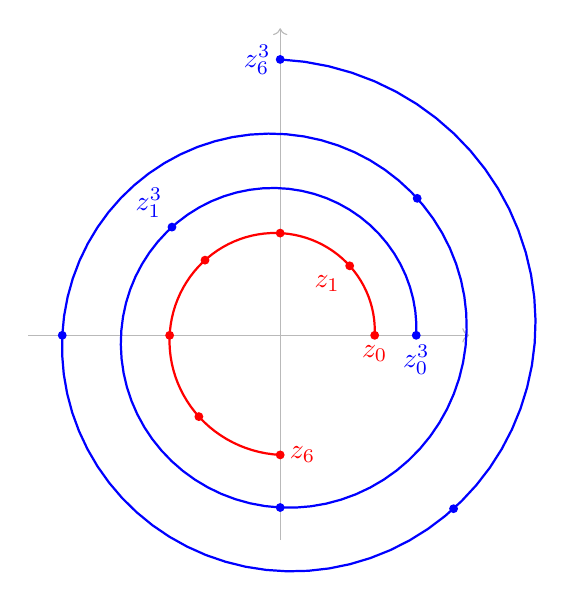
\begin{tikzpicture}[scale=1.0]
  % Complex plane axes.
  \draw[->, gray!55] (-3.2,0) -- (2.4,0);
  \draw[->, gray!55] (0,-2.6) -- (0,3.9);
  % Red arc: z(t) = 1.2 e^{0.05 t} (cos t, sin t), t in [0,270] degrees.
  \draw[red, thick, samples=80, domain=0:270, variable=\t]
    plot ({1.2*exp(0.05*\t*pi/180)*cos(\t)},
          {1.2*exp(0.05*\t*pi/180)*sin(\t)});
  % Blue arc: the cube, radius^3 and angle*3.
  \draw[blue, thick, samples=160, domain=0:270, variable=\t]
    plot ({pow(1.2*exp(0.05*\t*pi/180),3)*cos(3*\t)},
          {pow(1.2*exp(0.05*\t*pi/180),3)*sin(3*\t)});
  % Red sample points.
  \foreach \t in {0,45,...,270}
    \fill[red] ({1.2*exp(0.05*\t*pi/180)*cos(\t)},
                {1.2*exp(0.05*\t*pi/180)*sin(\t)}) circle (1.6pt);
  % Blue sample points (cubes).
  \foreach \t in {0,45,...,270}
    \fill[blue] ({pow(1.2*exp(0.05*\t*pi/180),3)*cos(3*\t)},
                 {pow(1.2*exp(0.05*\t*pi/180),3)*sin(3*\t)}) circle (1.6pt);
  % Labels.
  \node[red, below]      at (1.2,0)          {$z_0$};
  \node[red, below left] at ({1.248*cos(45)},{1.248*sin(45)}) {$z_1$};
  \node[red, right]      at (0,-1.519)       {$z_6$};
  \node[blue, below]      at (1.728,0)       {$z_0^3$};
  \node[blue, above left] at ({1.944*cos(135)},{1.944*sin(135)}) {$z_1^3$};
  \node[blue, left]       at (0,3.505)       {$z_6^3$};
\end{tikzpicture}
\end{document}
